\documentclass[]{article}
\usepackage{xcolor}
\usepackage{listings}
\usepackage{showexpl}
\usepackage{graphicx}
\usepackage[bahasai]{babel}
\lstset{language=Python,
	 numbers=left,
		stepnumber=1,
	numberstyle=\ttfamily,
	basicstyle=\ttfamily,
	keywordstyle=\color{blue}\ttfamily,
	stringstyle=\color{red}\ttfamily,
	commentstyle=\color{gray}\ttfamily,
	morecomment=[l][\color{magenta}]{\#},
    breaklines=true,
    %postbreak=\mbox{\textcolor{red}{$\hookrightarrow$}\space}
}


%opening
\title{Laporan Tugas 1}
\author{Akhmad Thoriq Afif NRP 5024201028}

\begin{document}
\maketitle
\section{Listing Program}
Berikut ini merupakan source code dari program mengganti background video.
\lstinputlisting[label={kodingan},caption={Listing Program}, language={Python}]{simple.py}
\section{Output Program}
\begin{figure}[H]
    \centering
    \includegraphics[width=12cm]{output.png}
    \caption{Output Program}
\end{figure}
\pagebreak
\section{Penjelasan Program}
\par
Pada program ini digunakan dua gambar sebagai foreground dan background.
\begin{figure}[H]
    \centering
    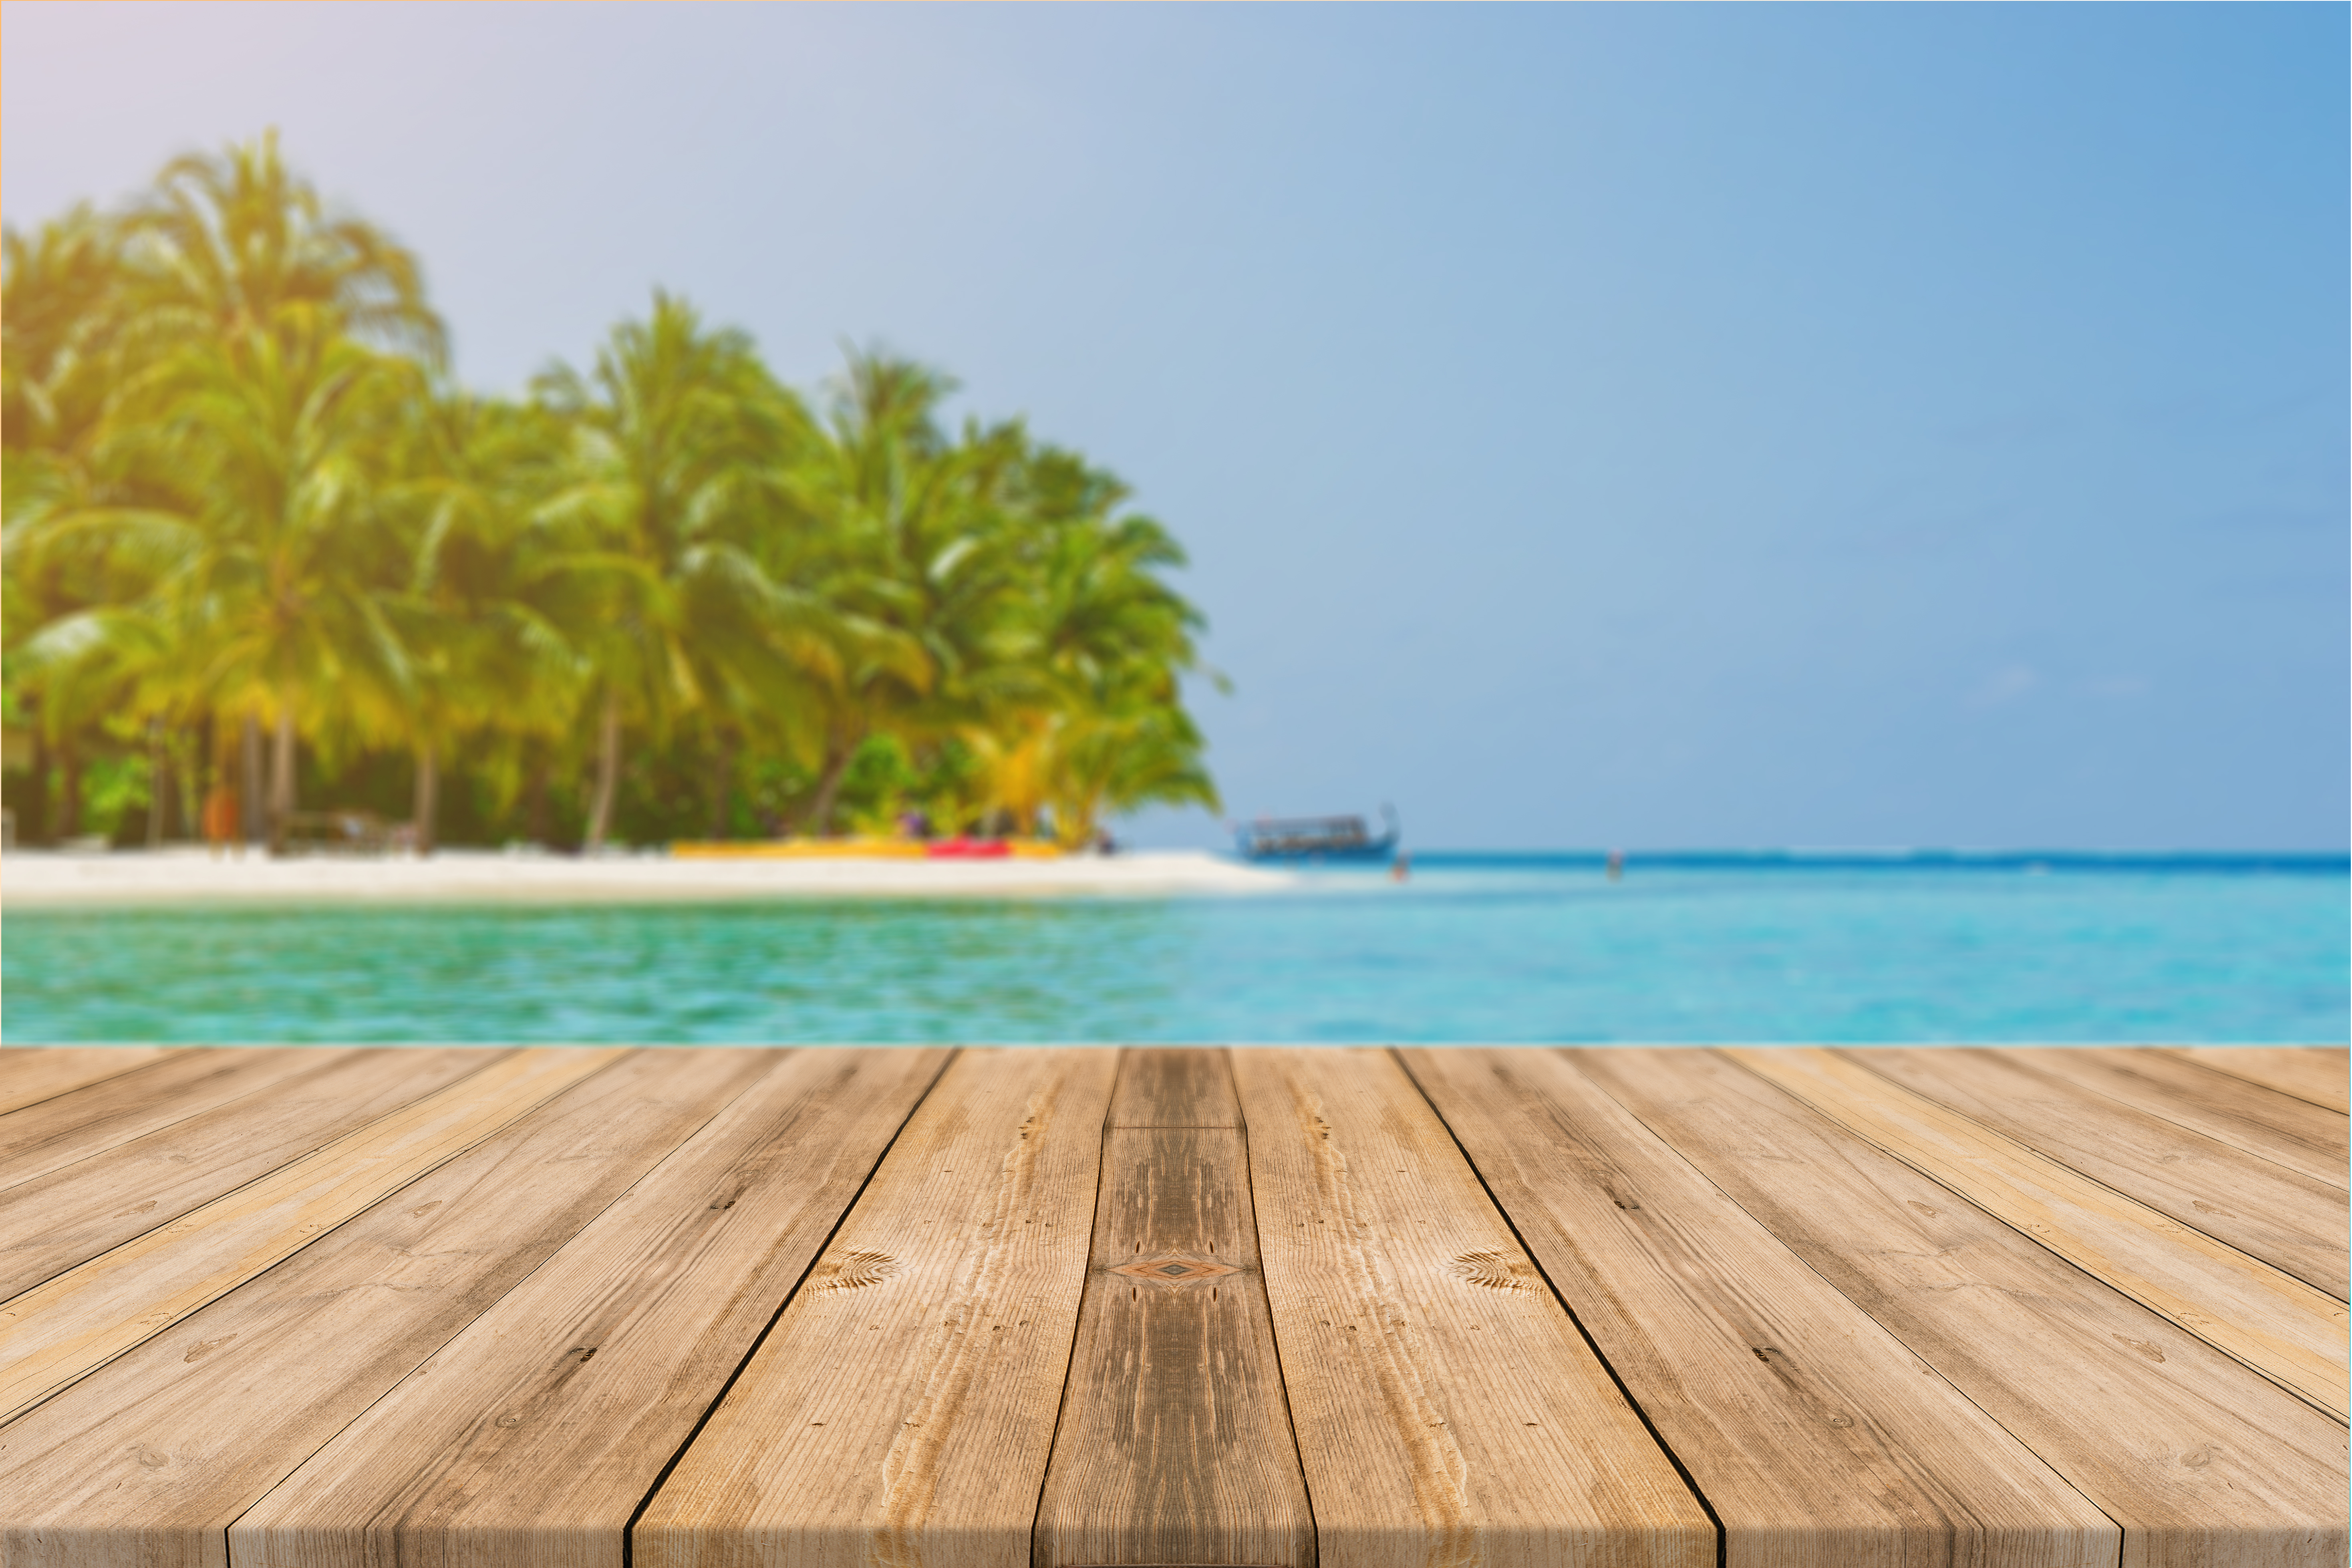
\includegraphics[width=12cm]{background.jpg}
    \caption{Gambar Background}
\end{figure}
\begin{figure}[H]
    \centering
    \includegraphics[width=12cm]{foreground.png}
    \caption{Gambar Foregound}
\end{figure}
\lstinputlisting[label={maxvalue},caption={Import library}, language={Python}, firstline=1, lastline=1]{simple.py}
Pada bagian awal program dilakukan import library yang digunakan yaitu library OpenCV
\lstinputlisting[label={maxvalue},caption={Penentuan lower dan upper bound}, language={Python}, firstline=3, lastline=4]{simple.py}
Kemudian ditentukan lower dan upper bound untuk warna yang akan dihilangkan pada background
Penentuan lower dan upper bound berdasarkan warna HSV
\begin{figure}[H]
    \centering
    \includegraphics[width=6cm]{hsvcolorwheel.png}
    \caption{HSV Colorwheel}
\end{figure}
\lstinputlisting[label={maxvalue},caption={Load background dan foreground}, language={Python}, firstline=6, lastline=7]{simple.py}
Kemudian background dan foreground diload menggunakan imread() untuk background (gambar) dan VideoCapture() untuk foreground (video)
\lstinputlisting[label={maxvalue},caption={Scalling ukuran background}, language={Python}, firstline=9, lastline=9]{simple.py}
Karena ukuran background terlalu besar dilakukan scalling untuk memperkecil ukuran menggunakan resize().
\lstinputlisting[label={maxvalue},caption={Blok while loop}, language={Python}, firstline=11, lastline=32]{simple.py}
Pada blok kode diatas proses manipulasi dilakukan. Karena pada program ini menggunakan video, maka digunakan while loop dengan batas True sehingga proses akan terus berlanjut hingga dilakukan break.
\lstinputlisting[label={maxvalue},caption={Pembacaan tiap frame video}, language={Python}, firstline=12, lastline=12]{simple.py}
Pada baris ini dilakukan pembacaan tiap frame video yang kemudian disiman pada variabel frame. Variabel ret akan digunakan untuk mengecek apakah video sudah mencapai akhir.
\lstinputlisting[label={maxvalue},caption={Pengeccekan frame video}, language={Python}, firstline=14, lastline=32]{simple.py}
Pada dua blok kode di atas dilakukan pengecekan apakah terdapat gambar pada frame. Jika tidak maka frame akan dikembalikan ke frame ke-0 sehingga akan terjadi loop pada video. Jika iya, proses manipulasi akan dilakukan.
\lstinputlisting[label={maxvalue},caption={Scalling ukuran foreground}, language={Python}, firstline=15, lastline=15]{simple.py}
Sama halnya dengan background pada foreground juga dilakukan scalling menjadi ukuran 640x360
\lstinputlisting[label={maxvalue},caption={Perubahan colorspace foreground menjadi HSV}, language={Python}, firstline=16, lastline=16]{simple.py}
Pada program ini digunakan HSV. Untuk mengubah colorspace foreground menjadi HSV digunakan cvtColor()
\begin{figure}[H]
    \centering
    \includegraphics[width=12cm]{hsv.png}
    \caption{Output HSV}
\end{figure}
\lstinputlisting[label={maxvalue},caption={Masking}, language={Python}, firstline=18, lastline=18]{simple.py}
Pada baris ini diambil semua warna yang berada diantara lower dan upper bound yang telah ditentukan. Hasilnya akan digunakan untuk memasking background.
\begin{figure}[H]
    \centering
    \includegraphics[width=12cm]{outputmask.png}
    \caption{Output Mask}
\end{figure}
\lstinputlisting[label={maxvalue},caption={Foreground Mask}, language={Python}, firstline=20, lastline=20]{simple.py}
Kemudian dibuat masking untuk foreground. Masking untuk foreground merupakan kebalikan dari masking untuk background, sehingga untuk membuatnya cukup membalikkan masking background dengan menggunakan bitwisenot.
\begin{figure}[H]
    \centering
    \includegraphics[width=12cm]{foregroundmask.png}
    \caption{Foreground Mask}
\end{figure}
\lstinputlisting[label={maxvalue},caption={Masking Foreground dan Background}, language={Python}, firstline=21, lastline=22]{simple.py}
Dari kedua mask tersebut dilakukan masking untuk foreground dan background dengan menggunakan bitwiseand. Hasil dari masking sebagai berikut
\begin{figure}[H]
    \centering
    \includegraphics[width=12cm]{foregroundmasked.png}
    \caption{Foreground Masked}
\end{figure}
\begin{figure}[H]
    \centering
    \includegraphics[width=12cm]{backgroundmasked.png}
    \caption{Background Masked}
\end{figure}
\lstinputlisting[label={maxvalue},caption={Menggabungkan foreground dan background}, language={Python}, firstline=24, lastline=26]{simple.py}
Dari hasil masking kemudian digabung menjadi satu menggunakan add(). Hasil penggabungan merupakan output dari program ini. Untuk menampilkan output digunakan imshow()
\begin{figure}[H]
    \centering
    \includegraphics[width=12cm]{outputakhir.png}
    \caption{Hasil Akhir}
\end{figure}




\end{document}